\documentclass{article}
\usepackage{amsfonts, amsthm, amsmath, amssymb, mathtools, ulem, mathrsfs, physics, esint, siunitx, tikz-cd}
\usepackage{pdfpages, fullpage, color, microtype, cancel, textcomp, markdown, hyperref, graphicx}
\usepackage{enumitem}
\usepackage{algorithm}
\usepackage{algpseudocode}
\graphicspath{{./images/}}
\usepackage[english]{babel}
\usepackage[autostyle, english=american]{csquotes}
\MakeOuterQuote{"}
\usepackage{xparse}
\usepackage{tikz}

\usepackage{calligra}
\DeclareMathAlphabet{\mathcalligra}{T1}{calligra}{m}{n}
\DeclareFontShape{T1}{calligra}{m}{n}{<->s*[2.2]callig15}{}
\newcommand{\script}[1]{\ensuremath{\mathcalligra{#1}}}
\newcommand{\scr}{\script r}

% fonts
\def\mbb#1{\mathbb{#1}}
\def\mfk#1{\mathfrak{#1}}
\def\mbf#1{\mathbf{#1}}
\def\tbf#1{\textbf{#1}}

% common bold letters
\def\bP{\mbb{P}}
\def\bC{\mbb{C}}
\def\bH{\mbb{H}}
\def\bI{\mbb{I}}
\def\bR{\mbb{R}}
\def\bQ{\mbb{Q}}
\def\bZ{\mbb{Z}}
\def\bN{\mbb{N}}

% brackets
\newcommand{\br}[1]{\left(#1\right)}
\newcommand{\sbr}[1]{\left[#1\right]}
\newcommand{\brc}[1]{\left\{#1\right\}}
\newcommand{\lbr}[1]{\left\langle#1\right\rangle}

% vectors
\renewcommand{\i}{\hat{\imath}}
\renewcommand{\j}{\hat{\jmath}}
\renewcommand{\k}{\hat{k}}
\newcommand{\proj}[2]{\text{proj}_{#2}\br{#1}}
\newcommand{\m}[2][b]{\begin{#1matrix}#2\end{#1matrix}}
\newcommand{\arr}[3][\sbr]{#1{\begin{array}{#2}#3\end{array}}}

% misc
\NewDocumentCommand{\seq}{O{n} O{1} O{\infty} m}{\br{#4}_{{#1}={#2}}^{#3}}
\NewDocumentCommand{\app}{O{x} O{\infty}}{\xrightarrow{#1\to#2}}
\newcommand{\sm}{\setminus}
\newcommand{\sse}{\subseteq}
\renewcommand{\ss}{\subset}
\newcommand{\vn}{\varnothing}
\newcommand{\lc}{\epsilon_{ijk}}
\newcommand{\ep}{\epsilon}
\newcommand{\vp}{\varphi}
\renewcommand{\th}{\theta}
\newcommand{\cjg}[1]{\overline{#1}}
\newcommand{\inv}{^{-1}}
\DeclareMathOperator{\im}{im}
\DeclareMathOperator{\id}{id}
\newcommand{\ans}{\tbf{Ans. }}
\newcommand{\pf}{\tbf{Pf. }}
\newcommand{\imp}{\implies}
\newcommand{\impleft}{\reflectbox{$\implies$}}
\newcommand{\ck}{\frac1{4\pi\ep_0}}
\newcommand{\ckb}{4\pi\ep_0}
\newcommand{\sto}{\longrightarrow}
\DeclareMathOperator{\cl}{cl}
\DeclareMathOperator{\intt}{int}
\DeclareMathOperator{\bd}{bd}
\DeclareMathOperator{\Span}{span}
\newcommand{\floor}[1]{\left\lfloor#1\right\rfloor}
\newcommand{\ceil}[1]{\left\lceil#1\right\rceil}
\newcommand{\fxn}[5]{#1:\begin{array}{rcl}#2&\longrightarrow & #3\\[-0.5mm]#4&\longmapsto &#5\end{array}}
\newcommand{\sep}[1][.5cm]{\vspace{#1}}
\DeclareMathOperator{\card}{card}
\renewcommand{\ip}[2]{\lbr{#1,#2}}
\renewcommand{\bar}{\overline}
\DeclareMathOperator{\cis}{cis}
\DeclareMathOperator{\Arg}{Arg}
\newcommand{\ptl}{\partial}
\newcommand{\Om}{\Omega}

% title
\title{Scientific Computing Final Exam}
\author{Ryan Chen}
%\date{\today}
\setlength{\parindent}{0pt}


\begin{document}
	
\maketitle

\section*{Problem 1}

\begin{enumerate}[label=(\alph*)]
	
\item
In this part we use the fact
$$\int_{-\infty}^{\infty}\exp(-ax^2+bx)dx = \br{\frac\pi a}^{1/2}\exp[\frac{b^2}{4a}]$$
Take the Fourier transform of the PDE in $x$, using the fact $\hat{\ptl_x^n\psi}=(i\xi)^n\psi$.
$$\hat\psi_t = \frac i2(i\xi)^2\hat\psi = -\frac i2\xi^2\hat\psi
\imp \hat\psi(\xi,t) = \hat\psi_0(\xi)\exp[-\frac i2\xi^2t]$$
Take the inverse Fourier transform.
$$\psi(x,t) = \frac{1}{(2\pi)^{1/2}}\int_{-\infty}^{\infty} \hat\psi_0(\xi)\exp[ix\xi - \frac i2t\xi^2]d\xi$$

Take the Fourier transform of the initial condition.
\begin{align*}
	\hat\psi_0(\xi) &= \frac{1}{(2\pi)^{1/2}}\frac{1}{(2\pi \sigma_0^2)^{1/4}}\int_{-\infty}^{\infty} \exp[-\frac{x^2}{4\sigma_0^2} + ik_0x - i\xi x]dx\\
	&= \frac{1}{(2\pi)^{3/4}\sigma_0^{1/2}}\int_{-\infty}^{\infty} \exp[-\frac{x^2}{4\sigma_0^2} + i(k_0-\xi)x]dx\\
	&= \frac{1}{(2\pi)^{3/4}\sigma_0^{1/2}}\pi^{1/2}2\sigma_0\exp[-(\xi-k_0)^2\sigma_0^2]\\
	&= \frac{2^{1/4}\sigma_0^{1/2}}{\pi^{1/4}}\exp[-(\xi-k_0)^2\sigma_0^2]
\end{align*}

Then
$$\psi(x,t) = \frac{1}{(2\pi)^{1/2}}\frac{2^{1/4}\sigma_0^{1/2}}{\pi^{1/4}}\int_{-\infty}^{\infty}\exp[-\sigma_0^2(\xi-k_0)^2 - \frac i2t\xi^2 + ix\xi]d\xi$$
Rewrite the argument of exp as
$$-\sigma_0^2(\xi-k_0)^2 - \frac i2t\xi^2 + ix\xi
= -\sigma_0^2(\xi^2+k_0^2-2k_0\xi) - \frac i2t\xi^2 + ix\xi
= -\br{\sigma_0^2 + \frac i2t}\xi^2 + (ix + 2\sigma_0^2k_0)\xi - \sigma_0^2k_0^2$$
so that
\begin{align*}
	\psi(x,t) &= \frac{\sigma_0^{1/2}}{2^{1/4}\pi^{3/4}}\int^{\infty}_{-\infty}\exp[-\br{\sigma_0^2 + \frac i2t}\xi^2 + (ix + 2\sigma_0^2k_0)\xi - \sigma_0^2k_0^2]d\xi\\
	&= \frac{\sigma_0^{1/2}}{2^{1/4}\pi^{3/4}}e^{-\sigma_0^2k_0^2}\br{\frac{\pi}{\sigma_0^2+\frac i2t}}^{1/2}\exp[\frac{-x^2 + 4\sigma_0^4k_0^2 + 4i\sigma_0^2k_0x}{4\br{\sigma_0^2 + \frac i2t}}]\\
	&= \frac{\sigma_0^{1/2}e^{-\sigma_0^2k_0^2}}{2^{1/4}\pi^{1/4}}\br{\sigma_0^2+\frac i2t}^{-1/2}\exp[\frac{-x^2 + 4\sigma_0^4k_0^2 + 4i\sigma_0^2k_0x}{4\br{\sigma_0^2 + \frac i2t}}]
\end{align*}


\item
Discretize the PDE in space with stepsize $h$ and use central differences.
$$\psi_j'(t) = \frac{i}{2h^2}[\psi_{j+1}(t) + u_{j-1}(t) - 2u_j(t)]$$
Let $v$ be such that $v(x_j,t)=\psi_j(t)$.
$$v_t(x,t) = \frac{i}{2h^2}[v(x+h,t) + v(x-h,t) - 2v(x,t)]$$
Taylor expand.
\begin{align*}
	v(x+h,t) &= v + hv_x + \frac12h^2v_{xx} + \frac16h^3v_{xxx} + \frac{1}{24}h^4v_{xxxx} + \frac{1}{120}h^5v_{xxxxx} + O(h^6)\\
	v(x-h,t) &= v - hv_x + \frac12h^2v_{xx} - \frac16h^3v_{xxx} + \frac{1}{24}h^4v_{xxxx} - \frac{1}{120}h^5v_{xxxxx} + O(h^6)
\end{align*}
Plug in the expansions.
$$v_t = \frac{i}{2h^2}\sbr{h^2v_{xx} + \frac{1}{12}h^4v_{xxxx} + O(h^6)}
= \frac i2v_{xx} + \frac{i}{24}h^2v_{xxxx} + O(h^4)$$
We obtain the (third order) modified equation.
$$v_t - \frac i2v_{xx} = \frac{i}{24}h^2v_{xxxx}$$
The Fourier transform of the RHS term is
$$\frac{i}{24}h^2\xi^4\hat v$$
so its corresponding term within the solution $\hat v(\xi,t)$ in Fourier space is
$$\exp[\frac{i}{24}h^2\xi^4t]$$
Thus the modified equation introduces artificial Fourier modes which do not decay over time.


\item
From now on we write $u$ instead of $\psi$.
\begin{algorithmic}
	\State pick maximum time $T$
	\State pick stepsize $h$ and timestep $k$
	\State set mesh using stepsize $h$
	\State $N \gets \frac Tk$
	\State set time points between 0 and $T$ using timestep $k$
	\State set initial condition vector $u_0$
	\State $\hat u_0 \gets$ DFT of $u_0$
	\State $\xi \gets 2\pi$ times vector of wavenumbers corresponding to mesh
	\State $\hat u \gets$ solution of PDE in Fourier space, $\hat u_t=-\frac i2\xi^2\hat u$ (use SciPy solver with $\hat u_0$ and set of time points)
	\State $u \gets$ array of 0s with the same size as $\hat u$
	\For{$j$th row of $u$}
		\State set the $j$th row of $u$ as the inverse DFT of the $j$th row of $\hat u$
	\EndFor
	\For{$j=0,\dots,N$}
		\If{$jk\in[0,t_1,\dots,t_M]$}
			\State print $j$th row of $u$
		\EndIf
	\EndFor
\end{algorithmic}

\end{enumerate}



\section*{Problem 2}

\begin{enumerate}[label=(\alph*)]
	
\item 

Code:

\url{https://github.com/RokettoJanpu/Scientific-Computing-2/blob/main/FINAL%20q2%20D02%2BRK4.ipynb}
\url{https://github.com/RokettoJanpu/Scientific-Computing-2/blob/main/FINAL%20q2%20DFT.ipynb}

In this part we take 4096 points in space. For $D_0^2$+RK4:
\begin{center}
	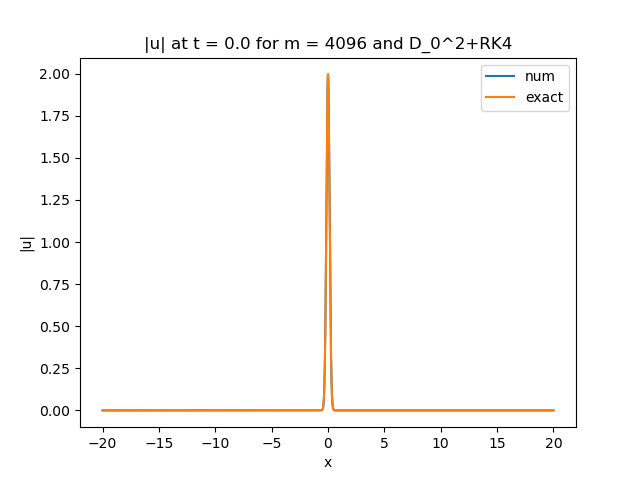
\includegraphics[scale=.3]{FINAL u_abs t = 0.0 m = 4096 D02+RK4}
	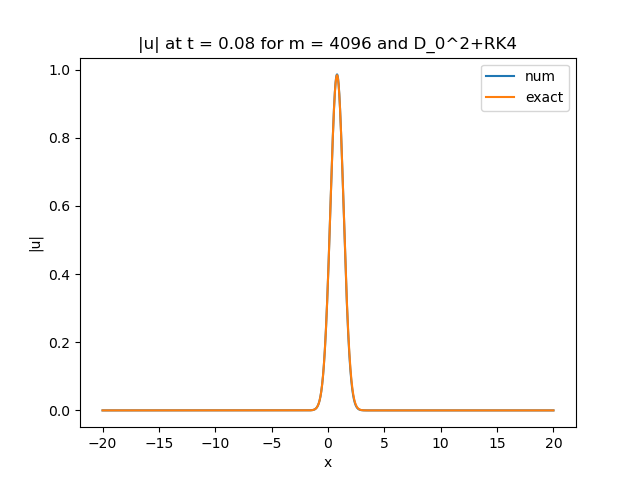
\includegraphics[scale=.3]{FINAL u_abs t = 0.08 m = 4096 D02+RK4}
	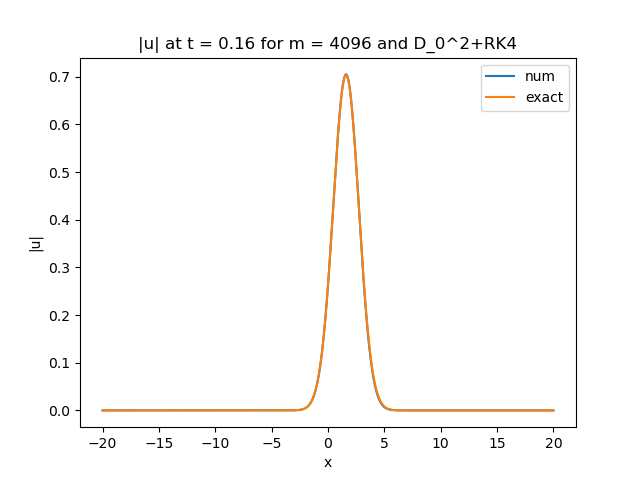
\includegraphics[scale=.3]{FINAL u_abs t = 0.16 m = 4096 D02+RK4}
\end{center}
\begin{center}
	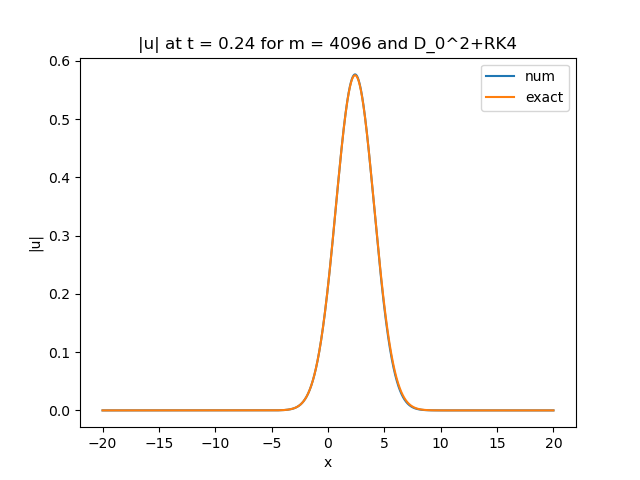
\includegraphics[scale=.3]{FINAL u_abs t = 0.24 m = 4096 D02+RK4}
	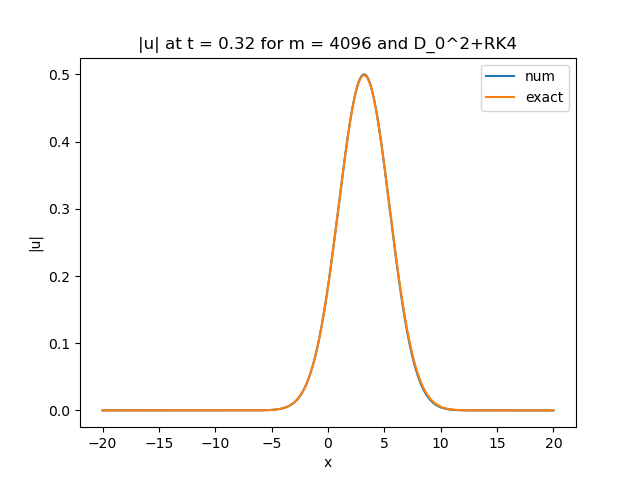
\includegraphics[scale=.3]{FINAL u_abs t = 0.32 m = 4096 D02+RK4}
	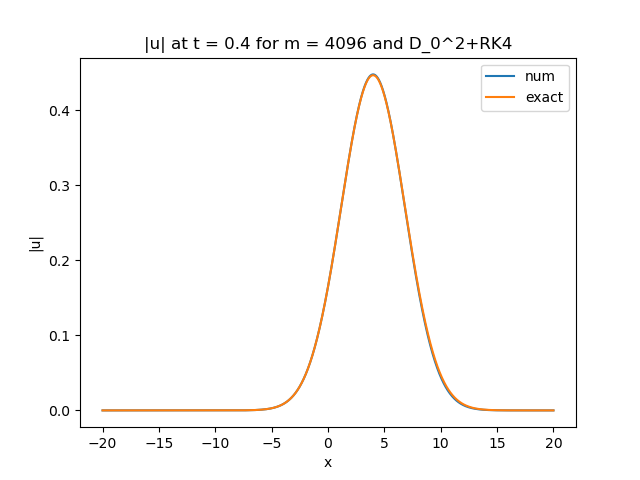
\includegraphics[scale=.3]{FINAL u_abs t = 0.4 m = 4096 D02+RK4}
\end{center}
We check the total probability is nearly equal to 1.
\begin{center}
	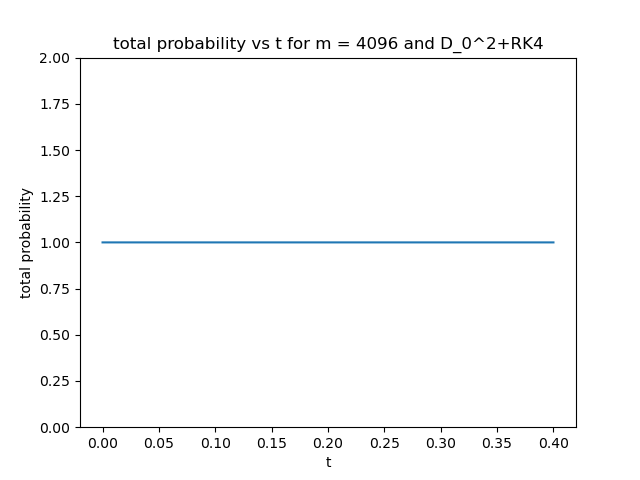
\includegraphics[scale=.5]{FINAL prob m = 4096 D02+RK4}
\end{center}
For the method using the discrete Fourier transform (DFT):
\begin{center}
	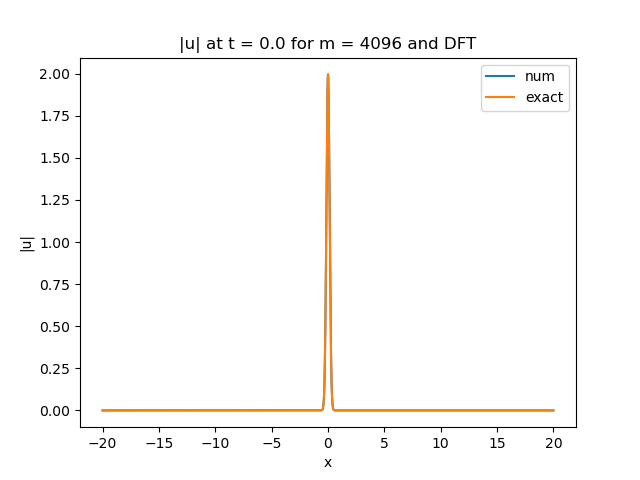
\includegraphics[scale=.3]{FINAL u_abs t = 0.0 m = 4096 DFT}
	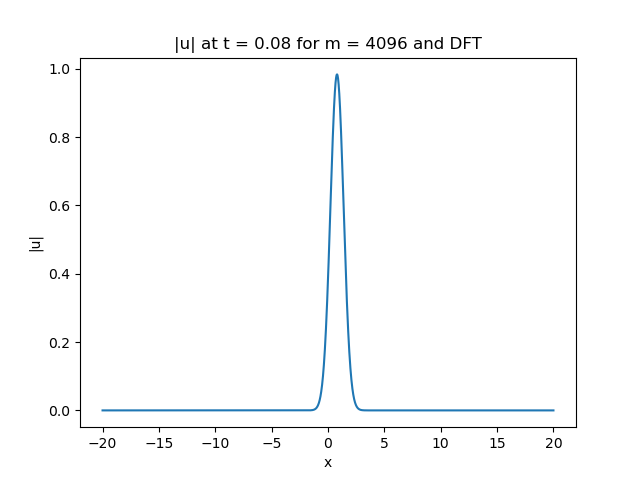
\includegraphics[scale=.3]{FINAL u_abs t = 0.08 m = 4096 DFT}
	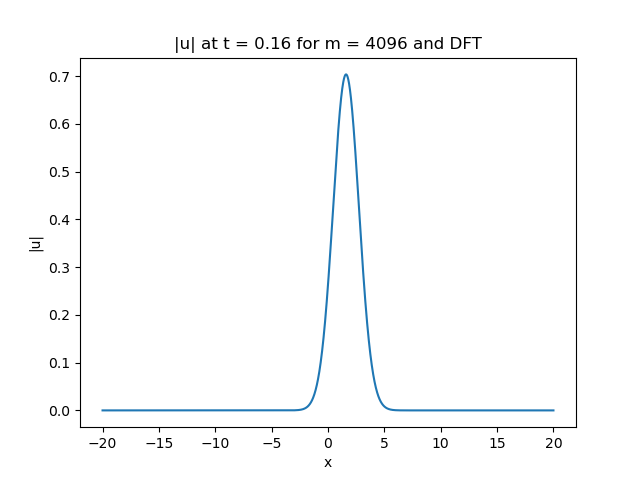
\includegraphics[scale=.3]{FINAL u_abs t = 0.16 m = 4096 DFT}
\end{center}
\begin{center}
	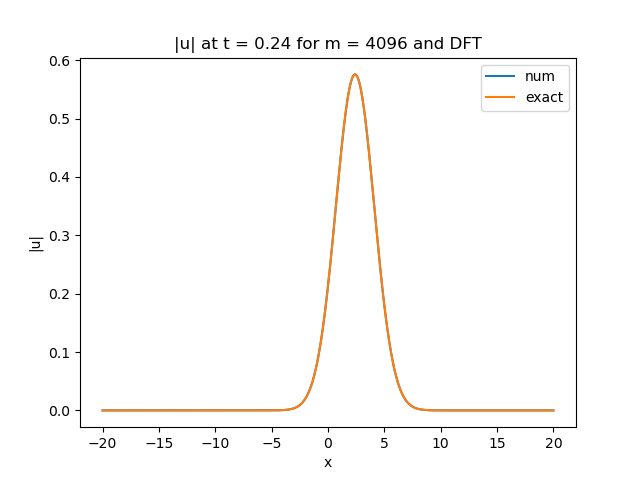
\includegraphics[scale=.3]{FINAL u_abs t = 0.24 m = 4096 DFT}
	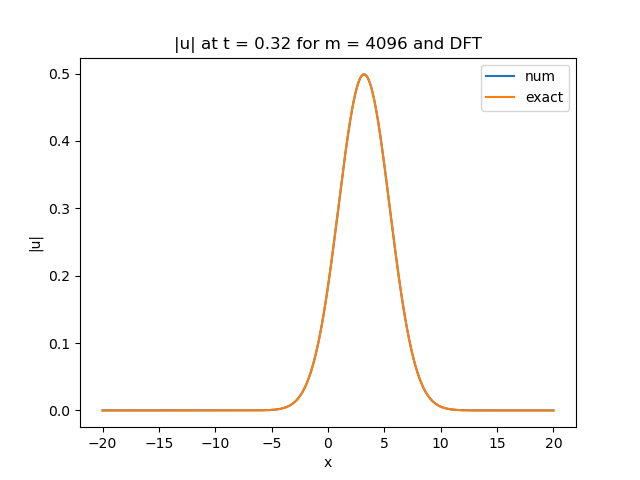
\includegraphics[scale=.3]{FINAL u_abs t = 0.32 m = 4096 DFT}
	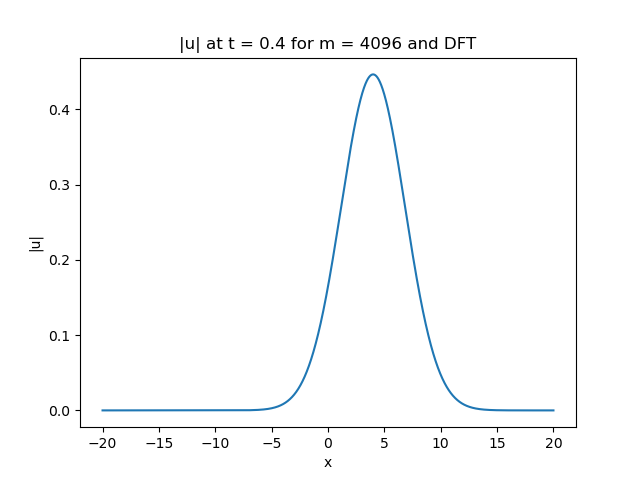
\includegraphics[scale=.3]{FINAL u_abs t = 0.4 m = 4096 DFT}
\end{center}
We check the total probability is nearly equal to 1.
\begin{center}
	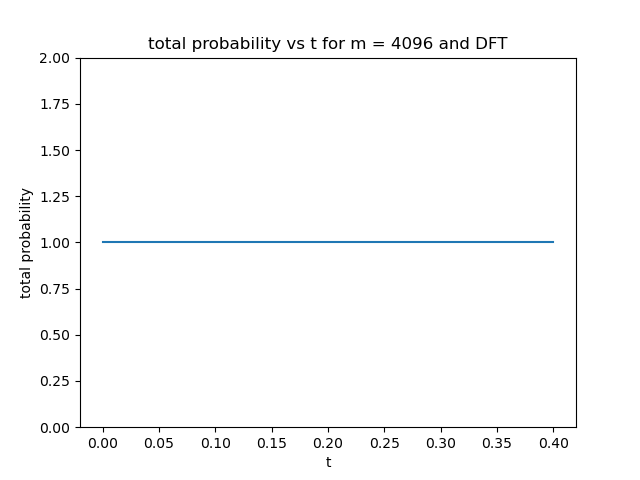
\includegraphics[scale=.5]{FINAL prob m = 4096 DFT}
\end{center}


\item 
In this part we take 256 points in space. For $D_0^2$+RK4:
\begin{center}
	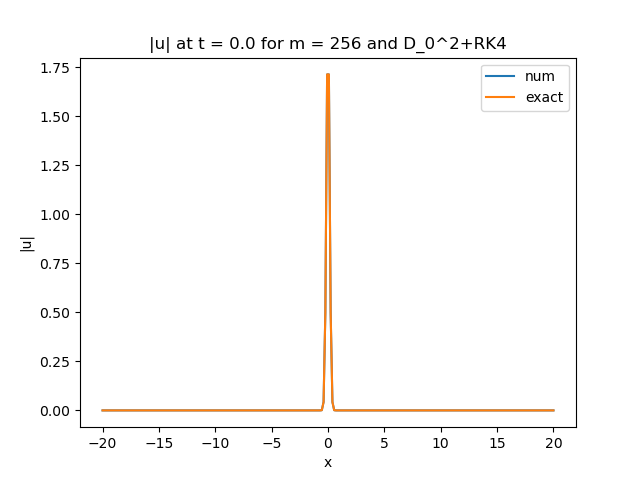
\includegraphics[scale=.3]{FINAL u_abs t = 0.0 m = 256 D02+RK4}
	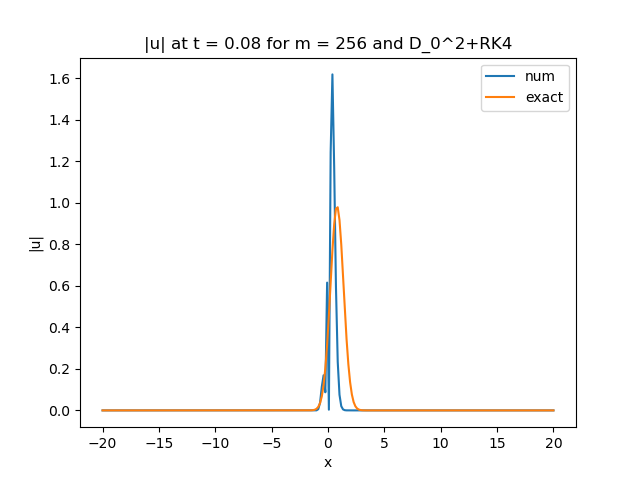
\includegraphics[scale=.3]{FINAL u_abs t = 0.08 m = 256 D02+RK4}
	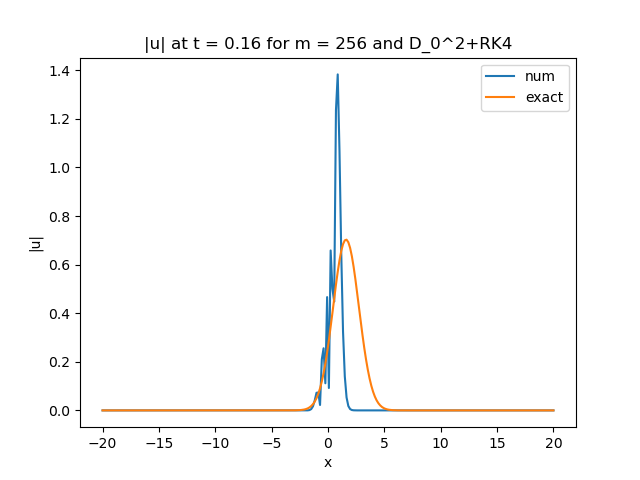
\includegraphics[scale=.3]{FINAL u_abs t = 0.16 m = 256 D02+RK4}
\end{center}
\begin{center}
	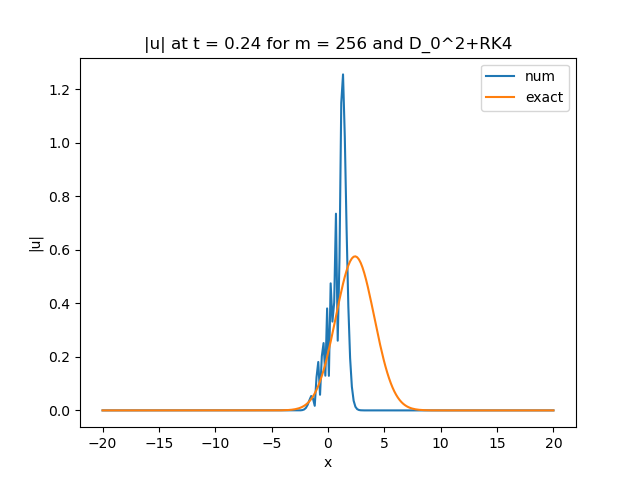
\includegraphics[scale=.3]{FINAL u_abs t = 0.24 m = 256 D02+RK4}
	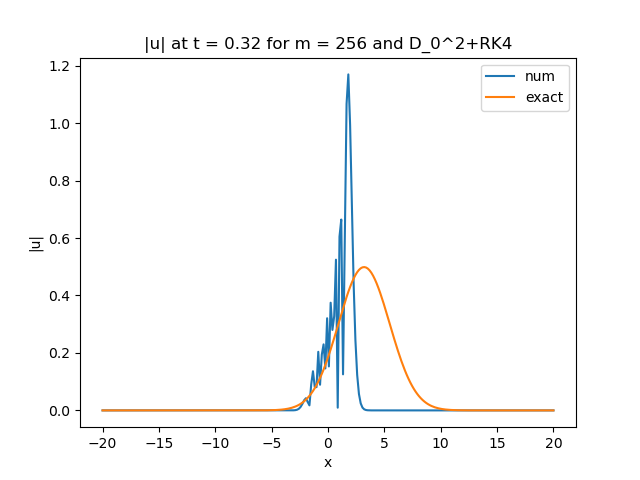
\includegraphics[scale=.3]{FINAL u_abs t = 0.32 m = 256 D02+RK4}
	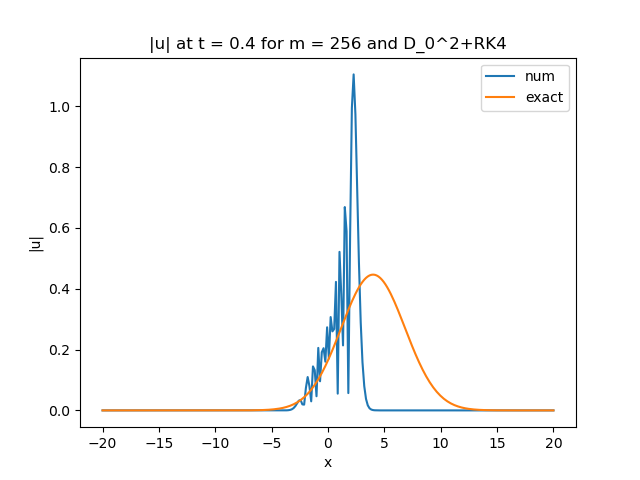
\includegraphics[scale=.3]{FINAL u_abs t = 0.4 m = 256 D02+RK4}
\end{center}
We check the total probability is nearly equal to 1.
\begin{center}
	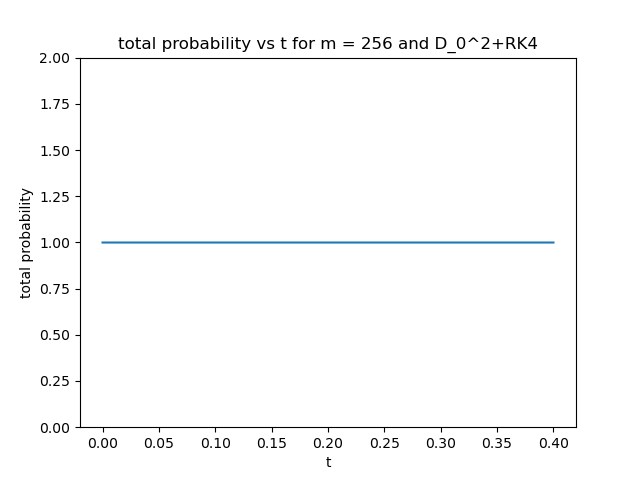
\includegraphics[scale=.5]{FINAL prob m = 256 D02+RK4}
\end{center}
For the method using the discrete Fourier transform (DFT):
\begin{center}
	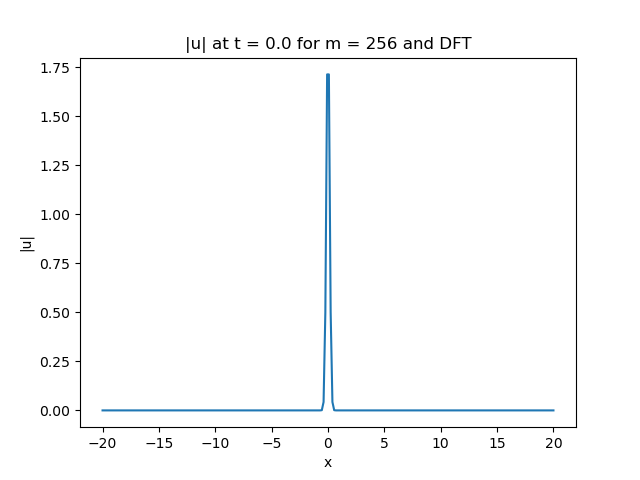
\includegraphics[scale=.3]{FINAL u_abs t = 0.0 m = 256 DFT}
	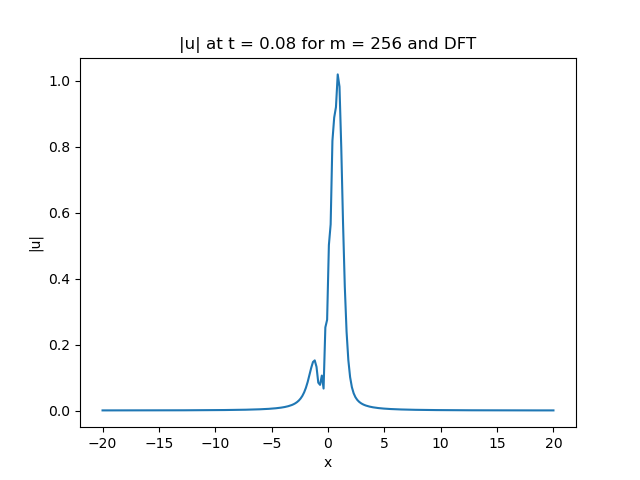
\includegraphics[scale=.3]{FINAL u_abs t = 0.08 m = 256 DFT}
	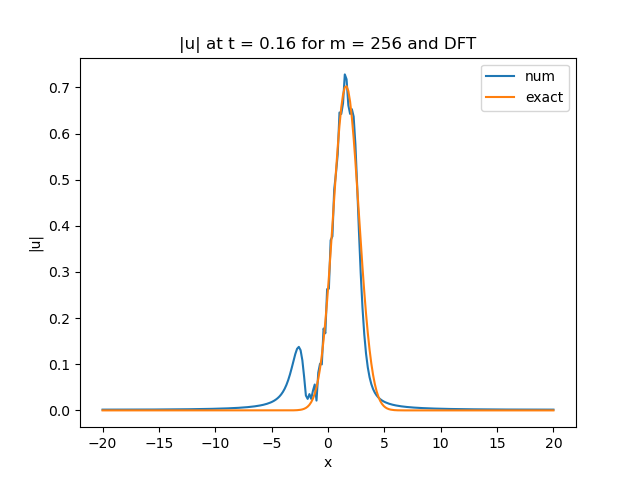
\includegraphics[scale=.3]{FINAL u_abs t = 0.16 m = 256 DFT}
\end{center}
\begin{center}
	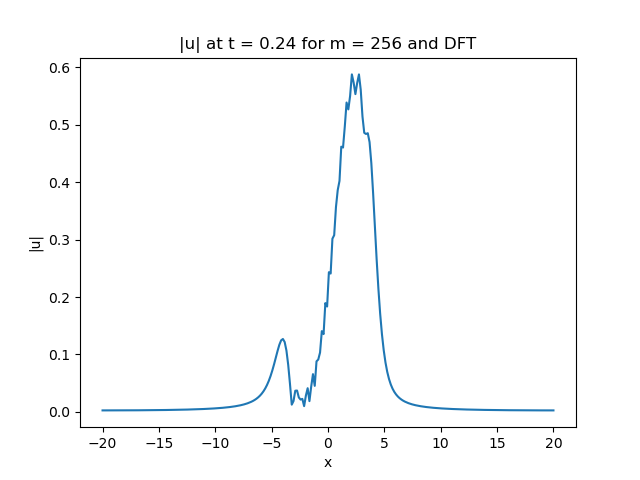
\includegraphics[scale=.3]{FINAL u_abs t = 0.24 m = 256 DFT}
	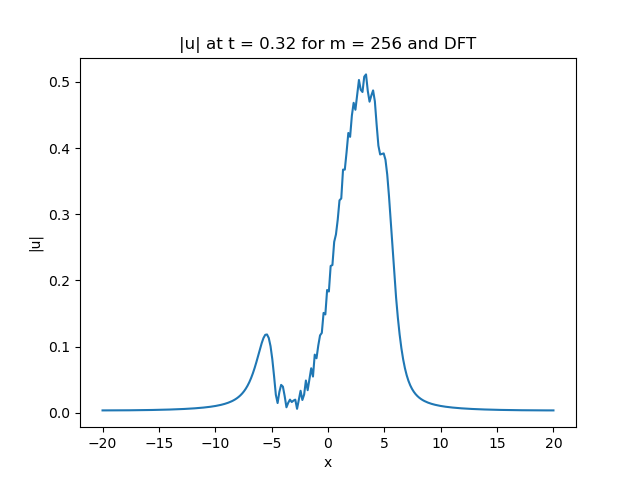
\includegraphics[scale=.3]{FINAL u_abs t = 0.32 m = 256 DFT}
	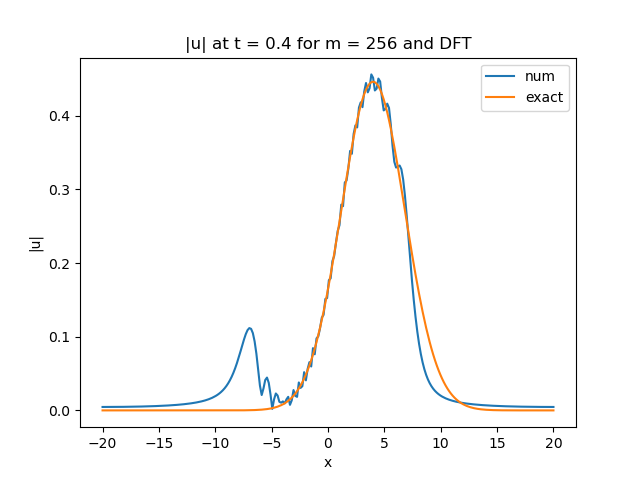
\includegraphics[scale=.3]{FINAL u_abs t = 0.4 m = 256 DFT}
\end{center}
We check the total probability is nearly equal to 1.
\begin{center}
	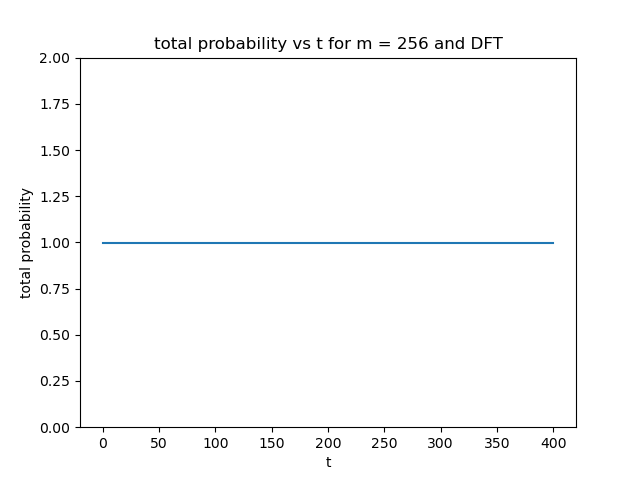
\includegraphics[scale=.5]{FINAL prob m = 256 DFT}
\end{center}

Recalling the modified equation for $D_0^2$+RK4, the error arises from artificial Fourier modes which do not decay over time. For DFT, the error arises from the splitting of the solution into Fourier modes of different propagation speeds.
	
\end{enumerate}


\section*{Problem 3}

\begin{enumerate}[label=(\alph*)]
	
\item
Fix a test function $v\in H_0^1(\Omega)$. Multiply the PDE by $v$ and integrate over $\Omega$.
$$\int_\Om \ep v\Delta udx = \int_\Om (u^3-u)vdx$$
Using Green's first identity and the fact $v=0$ on $\ptl\Om$, the LHS is
$$\int_\Om \ep v\Delta udx = -\int_\Om \ep\grad u\cdot\grad vdx + \int_{\ptl\Om} \ep v\pdv{u}{n}ds
= -\int_\Om \ep\grad u\cdot\grad vdx$$
Then we obtain the weak formulation.
$$-\int_\Om \ep\grad u\cdot\grad vdx = \int_\Om (u^3-u)vdx
\imp \int_\Om \ep\grad u\cdot\grad vdx - \int_\Om (u-u^3)vdx = 0$$


\item
Using Newton's iteration
$$y_{n+1} = y_n - J\inv(y_n)F(y_n)$$
we obtain
$$J\inv(y_n)F(y_n) = y_n - y_{n+1}
\imp F(y_n) = J(y_n)(y_n - y_{n+1})$$
Writing $y_n=(u^n,v)$ and casting $u^n-u^{n+1}$ as a parameter of $J$,
$$F(u^n,v) = J(u^n,v;u^n-u^{n+1})$$


\item
Code for problem 3:

\url{https://github.com/RokettoJanpu/Scientific-Computing-2/blob/main/FINAL%20q3.ipynb}

Below is a mesh of $\Omega$.

\begin{center}
	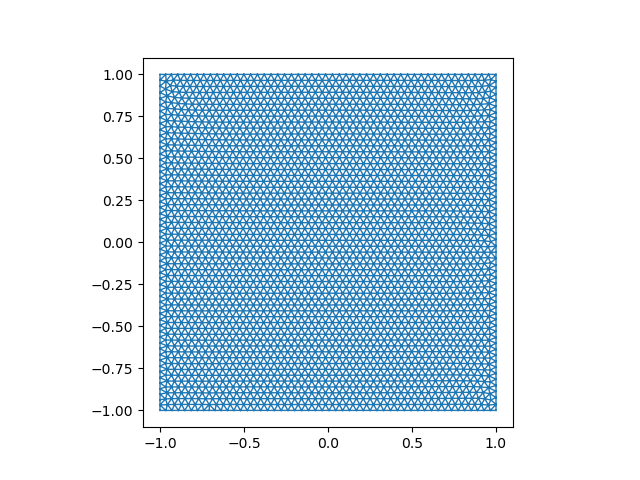
\includegraphics[scale=.5]{FINAL q3 mesh}
\end{center}
\end{enumerate}
	
\end{document}